\chapter{Monte Carlo Tree Search}
\label{MCTS}
In this chapter we present the second chosen algorithm \textit{Monte Carlo Tree Search}, giving a description of this algorithm and of its improvements which can be found in literature. We also present and briefly describe rules and complexity of Samegame, a puzzle domain where \textit{Monte Carlo Tree Search} achieve good results.

\medskip\noindent
Traditional artificial intelligence methods require a good heuristic function to evaluate moves and could be unsuitable for those domains in which defining an heuristic using expert knowledge is particularly difficult. In these situations, Monte Carlo methods can make up for the lack of a solid heuristic by obtaining an approximate evaluation of the game-theoretic value of a move, by relying on the use of simulated playouts. The value of action $a$ in state $s$ can be expressed as
\[Q(s,a) = \frac{1}{N(s,a)}\sum^{N(s)}_{i=1}I_i(s,a)z_i\]
Where $Q(s,a)$ is the action-value function, $N(s,a)$ is the number of times action $a$ has been selected from state $s$, $N(s)$ is the number of visits through state $s$, $I_i(s,a)$ has value 1 if action $a$ was selected from $s$ in the $i-th$ playout and $z_i$ is the final reward of simulation $i$. Essentially, the value of an action is computed as the average reward obtained in the playouts in which that action was taken.

\medskip\noindent
Monte Carlo evaluation was initially applied to tree search as an alternative to ad-hoc evaluation functions to prune the search tree \cite{10.1007/11674399_5} \cite{Juille99methodsfor}. These methods had the drawback of having no game-theoretic guarantees on the optimality of the solution.
Monte Carlo evaluation was also applied to Markov Decision Processes with better asymptotic properties \cite{doi:10.1287/opre.1040.0145} \cite{Bai:2015:OPL:2801030.2717316}. First visit Monte Carlo evaluation for example, is an unbiased estimator for the action-value function, meaning that given enough samples, it will converge to the actual function.

\medskip\noindent
The algorithm known as Monte Carlo Tree Search (MCTS) \cite{coulom:inria-00116992} was first proposed as an alternative to min-max trees with Monte Carlo evaluation and implemented in \textit{Crazy Stone}, a Go-playing program that won the 10th KGS computer-Go tournament. Over the years it has been successfully used in two-player zero-sum games with high branching factor like Go, Hex and Lines of Action \cite{gameExamples}.

\medskip\noindent
The next major step in MCTS development was the proposal of combining the \textit{Upper Confidence Bound} (UCB1) algorithm of Multi-Armed Bandit problems to MCTS. This created what we now know as \textit{Upper Confidence Bounds for Trees} (UCT) \cite{Kocsis:2006:BBM:2091602.2091633}. The UCB1 formula is used to balance exploration and exploitation during the tree search. Then, once reached a leaf node, a simulation is executed and the result is backpropagated to the root.
UCT is now the most used among the Monte Carlo methods. 

\section{State of the art}
Most of the research on MCTS has been carried out in the context of the game Go, an high branching factor two-players zero-sum game with no reliable heuristics for non-terminal positions. 
%The most successful Go implementations were only able to compete with intermediate level human players until recently. 
%
In 2016 Silver et al. \cite{Silver_2016} proposed a method that combined MCTS with convolutional neural networks and their program \textit{AlphaGo} was able to defeat 18-times human world champion Lee Sedol 4-1. They continued their research and while AlphaGo used expert knowledge to train the neural networks, their \textit{AlphaGo Zero} \cite{silver2017mastering} program was developed with no supervised learning, and was able to beat the original Alpha Go 100-0.

\medskip\noindent
Another board game in which MCTS has been successfully used is Hex that, unlike Go, has a robust evaluation function for the intermediate states; that is the reason why is possible to create good artificial intelligence using alpha-beta pruning
techniques \cite{journals/tciaig/ArnesonHH10}. In 2007, Arneson et al. \cite{journals/tciaig/ArnesonHH10} developed a program
based on Monte Carlo Tree Search, able to play the board game Hex. The program, called \textit{MoHex}, was able to win the silver and the gold medals at Computer Olympiads in 2008 and 2009 respectively, showing that it is able to compete with the artificial intelligence based on alpha-beta pruning.

\medskip\noindent
In the context of puzzle games, the research in MCTS methods is less developed and relatively recent. In the Samegame puzzle (Section \ref{sec:samegame}) the top score in a 20 levels set \cite{highscore} is currently held by tcooke with an undocumented method while the best score among documented algorithms was obtained by Edelkamp et al. with their \textit{Heuristically Guided Swarm Tree Search} \cite{Edelkamph} algorithm, a parallelized version of MCTS. Great results were also obtained by Schadd et al. \cite{DBLP:journals/kbs/SchaddWTU12} with a variant of the classic UCT algorithm called \textit{Single-Player Monte Carlo Tree Search}.

\medskip\noindent
Another puzzle in which MCTS methods excel is the Morpion solitaire. The current top scores of 178 and 82 respectively on the 5-T and 5-D versions of Morpion are held by Rosin and his \textit{Nested Rollout Policy Adaptation} \cite{IJCAI113358}, an extension of \textit{Nested Monte Carlo Search} \cite{Cazenave2009} in which the rollout policy is tuned adaptively starting from a uniform policy.

\medskip\noindent
Guez et al. \cite{DBLP:journals/corr/abs-1802-04697} proposed a method that combined neural networks and MCTS and trained it on the outcome of a MCTS algorithm on a set of very simple Sokoban levels ($10\times 10$ grid with a maximum of 4 boxes). As a result, after the offline supervised training, their method was able to reach the same performance as the baseline MCTS method but with far fewer iterations. The paper publication was eventually rejected due to the fact that the trained NN was considered to unlikely be able to generalize to other level configurations, in addition to the fact that the complete application of the method (offline and online phases) required far more resources than the baseline MCTS.
%TODO:search for more examples

\section{The Algorithm}\label{mctsalgorithm}
The MCTS algorithm builds an asymmetric search tree based on the results of Monte Carlo simulations. The tree growth is guided by the estimates it provides. It's an anytime algorithm, meaning that it can be stopped at any point in its execution and it will provide the best action for the root state so far. Its estimate values for the action become more precise as the algorithm continues its execution. The execution can be divided in four steps per iteration, as shown in Figure \ref{fig:MCTSsteps}:
\begin{enumerate}
    \item \textit{Selection}: starting from the root node, the algorithm recursively selects a child node according to some policy that should balance exploration and exploitation, until it reaches a node that has not been fully expanded, meaning not all of its moves lead to another node. The selection phase might also end if it reaches a terminal state;
    \item \textit{Expansion}: According to the expansion policy, one or more nodes - corresponding to the execution of the current node unexplored actions - are created and added to the tree;
    \item \textit{Rollout}: a simulated game is played, starting from the newly created node (the \textit{leaf node}), until a terminal state. This simulation is executed according to the default policy and it produces a reward;
    \item \textit{Backpropagation}: the reward obtained during the rollout phase is backpropagated through the tree, starting from the leaf node, upwards towards the root node. Each node contains the sum of the rewards of its children and the visit count (the number of times the node has been visited during the search).
\end{enumerate}

\begin{figure}[ht]
\begin{center}
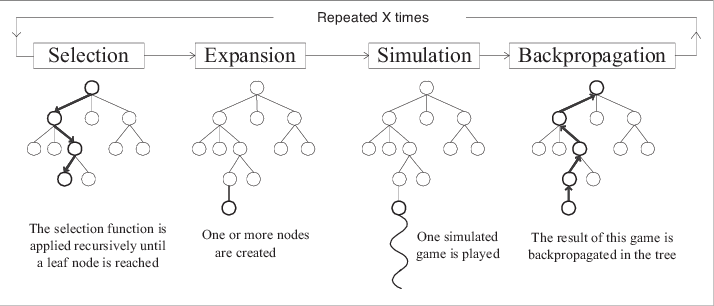
\includegraphics[width=\textwidth]{pictures/MCTSsteps.png}
\end{center}
\caption[MCTS steps]{Steps of the Monte Carlo tree search algorithm \cite{article}}
\label{fig:MCTSsteps}
\end{figure}

\medskip\noindent
The algorithm repeats this four steps until the end condition is met: this can be either a time constraint, a memory constraint or a limit in terms of number of iterations. At this point, the algorithm selects the best action for the root node according to a chosen criteria. Schadd \cite{bestcriteria} describes four
criteria for selecting the winning action, based on the work of
Chaslot et al. \cite{article}:
\begin{itemize}
    \item \textit{max child}: selects the child with the highest reward;
    \item \textit{robust child}: selects the most visited root child;
    \item \textit{max-robust child}: select the root child with both the highest visit count and the highest reward;
    \item \textit{secure child}: select the child which maximizes a lower confidence bound.
\end{itemize}
A MCTS algorithm is thus defined by the mentioned criterium, and by the policies used during the search. In the four steps of the algorithm we can identify four different policies:
\begin{itemize}
    \item \textit{Selection policy}: used to determine the way in which the tree is explored in the selection phase;
    \item \textit{Expansion policy}: used to determine which nodes are created in the expansion phase (usually one or all);
    \item \textit{Simulation policy}: used to determine the rollout behaviour. The usual default policy is a random policy, in which moves are sampled from a uniform distribution among those available in the current state, but often a policy handcrafted for the specific domain can obtain better performance;
    \item \textit{Backpropagation policy}: used to determine how the rewards are propagated in the tree. In the classical version of the method the reward is added to the sum of the rewards of a node and the number of visits is incremented.
\end{itemize}

\medskip\noindent
A general MCTS approach is summarized in Algorithm \ref{GeneralMCTS}. In this algorithm \textit{v\textsubscript{0}} is the root node corresponding to state \textit{s\textsubscript{0}}, \textit{v\textsubscript{l}} is the last node reached during the tree policy stage and corresponds to state \textit{s\textsubscript{l}}, and $\Delta$ is the reward for the terminal state reached by running the default policy from state \textit{s\textsubscript{l}}. The result of the overall search \textit{a}(\texttt{BESTCHILD}(\textit{v\textsubscript{0}})) is the action \textit{a} that leads to the best child of the root node \textit{v\textsubscript{0}}, where the exact definition of “best” is defined by the implementation.

\begin{algorithm}
  \caption[General MCTS approach]{\textbf{General MCTS approach}}\label{GeneralMCTS}
  \begin{algorithmic}
  \Function{MctsSearch}{$\textit{s\textsubscript{0}}$}
    \State create root node \textit{v\textsubscript{0}} with state \textit{s\textsubscript{0}}
    \While{within computational budget}
        \State $\textit{v\textsubscript{l}}\gets \Call{TreePolicy}{v\textsubscript{0}}$
        \State $\Delta\gets \Call{DefaultPolicy}{s(v\textsubscript{l}})$
        \State $\Call{Backup}{v\textsubscript{l}, \Delta}$
    \EndWhile
    \State \Return $\textit{a}(\Call{BestChild}{v\textsubscript{0}})$
    \EndFunction
  \end{algorithmic}
\end{algorithm}

\section{Upper Confidence Bounds for Trees}
Upper Confidence Bounds for Trees (UCT) is a version of the MCTS algorithm that uses UCB1 as a tree policy. The selection of a child node is therefore treated as a multiarmed bandit problem, in which the rewards correspond to random variables with unknown distributions. A child node i is thus selected to maximize
\begin{equation}\label{uctequation} 
UCT = \frac{v_i}{n_i} + C \times \sqrt{\frac{2\ln{n_p}}{n_i}} 
\end{equation}
where $v_i$ is the sum of the rewards obtained in all rollouts that have passed through node i, $n_i$ is number of times the node i (child of p) has been visited, $n_p$ is number of times the current node has been visited and $C$ is a constant used to balance exploration and exploitation. This formula is intrinsically balanced between the exploitation and exploration (represented respectively by the first and second term) as the number of visits of a node $n_i$ increases (inevitably together with $n_p$), the second term decreases, while when another child of the same parent node is visited, only $n_p$ in the numerator increases.
The constant value can be adjusted to favor exploration or exploitation. The value of $C=1$ was shown to ensure the asymptotic optimality of the solution with rewards the range [0,1] \cite{Kocsis2006ImprovedMS}. With rewards outside this range, appropriate values of $C$ could be found by manual tuning or other automated method \cite{Rubinstein1999}. Algorithm \ref{UCTalgorithm} shows the UCT algorithm in pseudocode.

\begin{algorithm}
  \caption[UCT Algorithm]{\textbf{UCT Algorithm}}\label{UCTalgorithm}
  \begin{algorithmic}
  \Function{UctSearch}{$\textit{s\textsubscript{0}}$}
    \State create root node \textit{v\textsubscript{0}} with state \textit{s\textsubscript{0}}
    \While{within computational budget}
        \State $\textit{v\textsubscript{l}}\gets \Call{TreePolicy}{v\textsubscript{0}}$
        \State $\Delta\gets \Call{DefaultPolicy}{s(v\textsubscript{l}})$
        \State $\Call{Backup}{v\textsubscript{l}, \Delta}$
    \EndWhile
    \State \Return $\textit{a}(\Call{BestChild}{v\textsubscript{0}, 0})$
    \EndFunction
    
    \Function{TreePolicy}{$v$}
    \While{\textit{v} is nonterminal}
        \If{\textit{v} not fully expanded}
        \State \Return $\Call{Expand}{v}$
        \EndIf
        \State \textbf{else}
        \State \hspace{\algorithmicindent}$v\gets \Call{BestChild}{v, C\textsubscript{p}}$
    \EndWhile
    \State \Return $v$
    \EndFunction
    
    \Function{Expand}{$v$}
    \State choose \textit{a} $\in$ untried actions from \textit{A}(\textit{s}(\textit{v}))
    \State add a new child \textit{v'} to \textit{v}
    \State \hspace{\algorithmicindent} with \textit{s}(\textit{v'}) = \textit{f}(\textit{s}(\textit{v}), \textit{a})
    \State \hspace{\algorithmicindent} and \textit{a}(\textit{v'}) = \textit{a}
    \State \Return \textit{v'}
    \EndFunction
    
    \Function{BestChild}{$v, c$}
    \State \Return $\argmax\limits_{v' \in \,children\,of\,v} \frac{Q(v')}{N(v')} + c \times \sqrt{\frac{2\ln{N(v)}}{N(v')}}$
    \EndFunction
    
    \Function{DefaulPolicy}{$s$}
    \While{\textit{s} is non-terminal}
        \State choose \textit{a} $\in$ \textit{A}(\textit{s}) uniformly at random
        \State $s\gets f(s, a)$
    \EndWhile
    \State \Return reward for state \textit{s}
    \EndFunction
    
    \Function{Backup}{$v, \Delta$}
    \While{\textit{v} is non null}
        \State $N(v)\gets N(v) + 1$
        \State $Q(v)\gets Q(v) + \Delta(v, p)$
        \State $v\gets$ parent of $v$
    \EndWhile
    \EndFunction
  \end{algorithmic}
\end{algorithm}

\medskip\noindent
Each node \textit{v} contains information about: the associated state \textit{s}(\textit{v}), the outgoing action \textit{a}(\textit{v}), the total simulation reward \textit{Q}(\textit{v}) and the visit count \textit{N}(\textit{v}). To have a more efficient usage of memory, the associated state \textit{s}(\textit{v}) is recomputed as \texttt{TREEPOLICY} descends the tree, instead of storing it for each node. The term $\Delta(v,p)$ in function \texttt{BACKUP} indicates the component of the reward vector $\Delta$ associated with the current player \textit{p} at node \textit{v}. The return value of the overall search is given by \textit{a}(\texttt{BESTCHILD}(\textit{v\textsubscript{0}})), that is the action \textit{a} associated to the child which has the highest reward, due to the fact that the exploration parameter \textit{c} is set to 0 for the final call of this function on the root node \textit{v\textsubscript{0}}.

\section{Characteristics}
MCTS is a popular choice of algorithm for a variety of domains due to three main characteristics:
\begin{enumerate}
    \item \textit{Analytic}: MCTS does not require any domain-specific knowledge, it is sufficient to know only its legal moves and end conditions. This makes it applicable to any domain that can be modeled using a tree. However, in its basic version, MCTS can have low performance and some domain-specific knowledge can be included in order to significantly improve the speed of the algorithm;
    \item \textit{Anytime}: MCTS backpropagates the outcome at the end of every iteration, so the whole tree is immediately updated with the last calculated rewards and visits counts. This allows the algorithm to stop and return the current best root action at any moment in time. Allowing the algorithm to run for extra iterations often improves the result;
    \item \textit{Asymmetric}: The tree policy allows the algorithm to use more computational resources on the most promising nodes of the tree, leading to an asymmetric growth of it over time. This makes the tree adapt to the topology of the search space leading to a better understanding about the game itself and making MCTS suitable for games with high branching factor.
\end{enumerate}

\section{MCTS Enhancements}
A huge number of enhancements have been proposed for the core MCTS algorithm in order to improve performance, including modifications of the tree policy, the default policy and other more general modifications related to the backpropagation step and parallelization as described in Cameron et al. work \cite{journals/tciaig/BrownePWLCRTPSC12}. These enhancements can generally be divided into two categories: \textit{Domain independent} enhancements that do not require any prior knowledge about the domain in order to be applied in it; \textit{Domain dependent} enhancements that are specific to particular domains. A more specific categorization can be done considering the used approach.

\subsubsection{Bandit-Based Enhancements}
This approach modifies the bandit-based method used for node selection in the tree policy. For this kind of enhancements plenty of different upper confidence bounds have been proposed, often improving bounds or performances in particular circumstances.

\subsubsection{Selection Enhancements}
This approach modify the tree policy in order to change how MCTS explores the search tree. The basic idea of selection is to assign a numeric score to each action in order to balance exploration with exploitation, so these enhancements influence this score using some domain knowledge in order to bias the search toward the most promising area and make use of different kind of reward estimation.

\subsubsection{All Moves As First (AMAF)}
This approach modifies how node statistics are updated. The basic idea is to update statistics for all action that are selected during a rollout as if they were the first action applied. The AMAF algorithm treats all moves played during selection and rollout steps as if they were played on a previous selection step, meaning that the reward estimate for an action \textit{a} from a state \textit{s} is updated whenever \textit{a} occurs during a playout, even if \textit{a} was not the actual move chosen from \textit{s}.

\subsubsection{Game-Theoretic Enhancements}
This approach uses the known game-theoretic value of a state to improve reward estimates for other non-terminal nodes backpropagating it up the tree.

\subsubsection{Move Pruning}
This approach applies the pruning technique, already used with \textit{minimax}, in order to eliminate obviously poor choices and allow the search to focus more resources on the better ones.

\subsubsection{Simulation Enhancements}
This approach modifies the default simulation policy for MCTS which select randomly among the available actions, trying to obtain more realistic simulations by incorporating domain knowledge into the playouts.

\subsubsection{Backpropagation Enhancements}
This approach modifies the backpropagation step involving special node updates.

\subsubsection{Parallelization Enhancements}
This approach exploit the independent nature of each simulation in MCTS to introduce parallization. More simulations can be performed in a given amount of time and the wide availability of multicore processors can be exploited. However, parallelization raises issues such as the combination of results from different sources in a single search tree, and the synchronization of threads of different speeds over a network.

\section{MCTS for puzzles}\label{sec:spmcts}
UCT was initially proposed for two-player games, therefore --- as in minimax and other adversarial search algorithms --- some of its characteristics were based on the assumption that there was a second player with the goal of minimizing our reward. Schadd et al. \cite{DBLP:journals/kbs/SchaddWTU12} presented a variant called \textit{Single-Player Monte-Carlo Tree Search} (SP-MCTS) in which they exploit some properties of single-player games to increase the effectiveness of MCTS. The core mechanism of SP-MCTS is the same as in UCT. One of the new ideas introduced is a variation the selection strategy, which aims to maximize the following formula:
\begin{equation}\label{spmctsequation}
    SP-UCT = \frac{v_i}{n_i} + C \times \sqrt{\frac{2\ln{n_p}}{n_i}} +\sqrt{\frac{\sum{v_i^2} - n_i \times (\frac{v_i}{n_i})^2 + D}{n_i}}
\end{equation} 
where the first two terms represent the UCT formula \ref{uctequation}, while the newly added term represents possible deviations in the child node scores. Using the same notation used in the UCT formula, $\sum{v_i^2}$ is the sum of squared rewards obtained by rollouts that have transited through node $n_i$, $n_i \times (\frac{v_i}{n_i})^2$ is the expected squared reward, $D$ is a large constant used to ensure that rarely explored nodes are considered promising.

\medskip\noindent
One of the aspects in which puzzles can differ from zero-sum two-player games is the range of values for the reward. While in two-player games the outcome is usually defined as \{0, $\frac{1}{2}$, 1\} or \{-1, 0, 1\} for loss, draw or win, in puzzles where the goal is to maximize the score the reward can vary greatly in range. Keeping in mind that \cite{DBLP:journals/kbs/SchaddWTU12} chose Samegame as a case study (which has a score in the order of thousands), the third term of the formula was specifically designed to take advantage of the score variation. Another major difference from two-player games is the absence of an opponent. The consequence is that if the game is deterministic there is no uncertainty given by the opponent choices. This leads to the second variation introduced in SP-MCTS: the method to choose the root action at the end of the search is not one of the four mentioned in Section \ref{mctsalgorithm} which generally aim towards the maximization of the winning probability, but instead the selected action is the one that belongs to the path which maximizes the top score. In order to employ this policy and to evaluate equation \ref{spmctsequation} the backpropagation policy was slightly modified to store in the nodes additional information like the total squared rewards and the top score. The best solution, i.e. the one with the highest score, was also stored throughout the search to ensure that the final result is the best among all rollouts executed.

\medskip\noindent
Schadd et al. \cite{DBLP:journals/kbs/SchaddWTU12} also applied a single-threaded version of root parallelization \cite{10.1007/978-3-540-87608-3_6} called \textit{Randomized Restarts} in which the search is repeated multiple times with different random seeds to avoid getting caught in local optima.
They used the \textit{Cross Entropy Method} \cite{Rubinstein1999} to tune the parameters and managed to obtain a score of 78012 in a standardized Samegame test set.

\subsection{Samegame}\label{sec:samegame}
Samegame is a fully observable deterministic single player game invented by Kuniaki Moribe under the name \textit{ChainShot!} in 1985.  In 1992 Eiji Fukumoto ported the game to Unix with a slight variation in settings calling it Samegame. Samegame is a tile-matching game and numerous variations of the game have been developed over the years.

\subsubsection{Rules}
Samegame is played on an $n\times m$ grid containing randomly arranged blocks of $k$ different colors. The goal of the game is to obtain the highest score by removing groups of blocks. At every move, the player can remove a group of two or more orthogonally adjacent blocks of the same color. Once a block has been removed, all blocks above it in the same column will slide down until there are no holes left, as if they were subject to gravity, as shown in Figure \ref{fig:samegame_b}. Once an entire column is removed, all columns on its right will slide to the left until there are no empty columns left, as shown in Figure \ref{fig:samegame_c}.

\begin{figure}[ht]
\label{fig:samegameexample}
\centering
\subfigure[Playing move (C,3)]{
\label{fig:samegame_a}
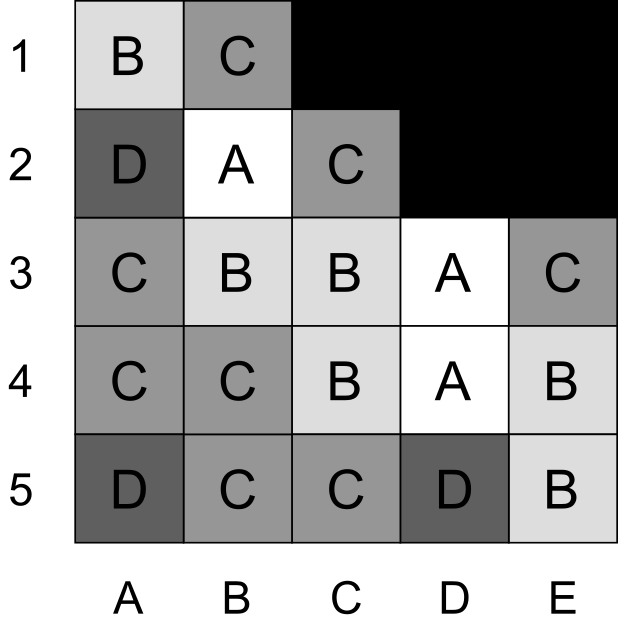
\includegraphics[width=0.28\linewidth]{pictures/samegame_a.png}}
\quad
\subfigure[Playing move (C,4)]{
\label{fig:samegame_b}
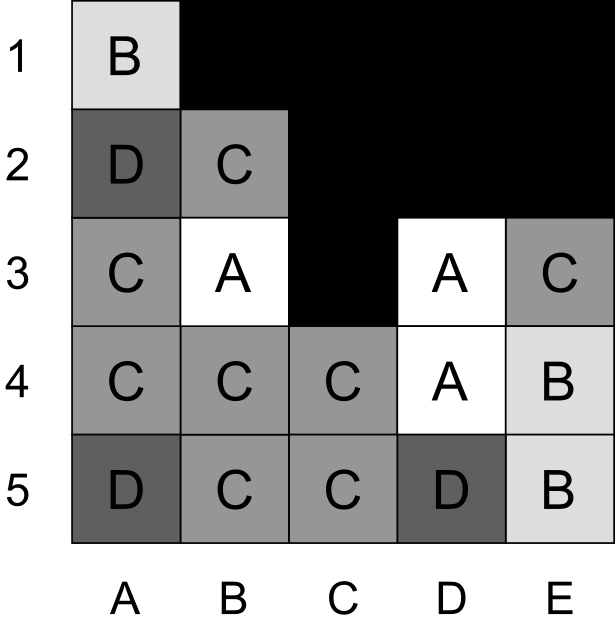
\includegraphics[width=0.28\linewidth]{pictures/samegame_b.png}}
\quad
\subfigure[Result]{
\label{fig:samegame_c}
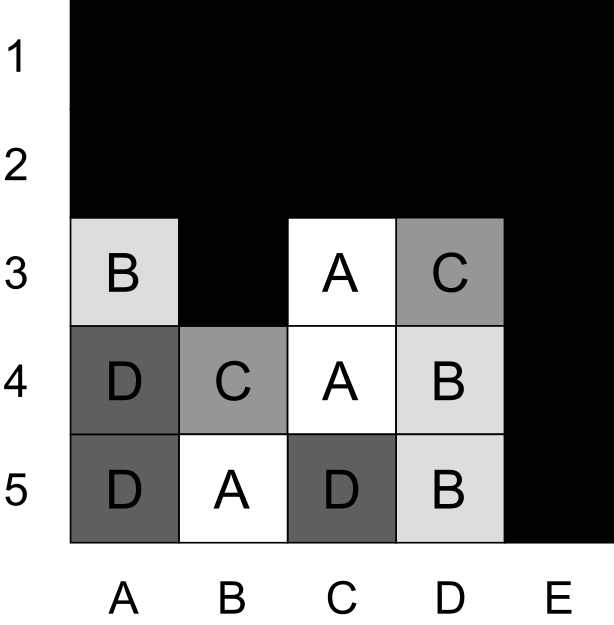
\includegraphics[width=0.28\linewidth]{pictures/samegame_c.png}}
\caption[Move sequence example]{Move sequence example \cite{DBLP:journals/kbs/SchaddWTU12}}
\end{figure}

\medskip\noindent
Points are rewarded for each action according to the formula $(n-2)^2$, where $n$ is the number of blocks removed with the current action. The game is over when either the player has cleared the board, leaving no blocks behind, or there are no more legal moves left, meaning that there are no two blocks with the same color are adjacent to each other.\\
Final points are awarded or subtracted based on the above end game condition: 
\begin{itemize}
    \item If the player was able to clear the board: A bonus of 1000 points is awarded.
    \item If the player was unable to clear the board: Points are subtracted using the formula $\sum{(n_i-2)^2}$ where $n_i$ is the number of blocks of the same color still on the board.
\end{itemize}
The standard game configuration is a $15\times 15$ board with $5$ colors. Given the scoring system, the maximum theoretical achievable score is $(n\times m-2)^2 +1000$, with $n$ and $m$ being rows and columns. With the standard configuration this results in a total of 49829. This is only obtainable if the initial configuration contains only a single color, requiring that no constraint on the minimum number of colors present are applied. If we consider enforcing the presence of all 5 colors, the maximum score becomes 48861. However, the actual score for a randomly generated board is rarely higher than 6000 points. On the 20 levels standard test set used in most researches \cite{DBLP:journals/kbs/SchaddWTU12} \cite{Cazenave2009} \cite{IJCAI113358}, the average score of the best algorithm is 4392.1 \cite{highscore}.

\medskip\noindent
The same mechanics can be found in other games, with the only difference often being the scoring formula. In \textit{Clickomania!} for example the objective is minimizing the number of blocks remaining, thus clearing the board represent the top score. In \textit{Jawbreaker}, a the Samegame porting for Microsoft Windows Mobile 2003, the formula used is $n(n-1)$, while in the Windows 3.1 porting the game is still called Samegame, but it computes the score as $n^2-3n+4$.

\subsubsection{Complexity}
A good estimator for the complexity of a game is the game-tree complexity, that represents the number of leaf nodes in the search tree and can be approximated by $b^d$, where $b$ is the average branching factor and $d$ is the average game length. In Samegame the player can choose a block as a move and in a $15\times 15$ board that would lead to an initial branching factor of 225. In reality, all moves in the same block group are equivalent so the actual branching factor is normally smaller. It also generally decreases as the game progresses. Schadd et al. \cite{DBLP:journals/kbs/SchaddWTU12} calculated the average game length and the average branching factor over 250 different configurations, and obtained $d=62.2$ and $b=21.1$, resulting in a game-tree complexity of $10^{82}$.Another estimator for the complexity can be the state-space complexity, which is the total number of legal board configurations reachable from the initial state. In the case of Samegame, it can be computed as $C^m$ where $m$ is the number of columns and $C$ is the number of possible configurations of a single column, obtained as $C=\sum_{i=0}^n{k^i}$, where n is the number of rows and k is the number of different colors. With $n=15$, $m=15$ and $k=5$ we can obtain a state-space complexity of $10^{159}$. Furthermore, Samegame has been proven to be at least of complexity class NP-complete \cite{DBLP:journals/kbs/SchaddWTU12}.

\medskip\noindent
In addition to the sheer values of game-tree and state-space complexity - that render uninformed search methods unfeasible - it's very hard to find a reliable admissible heuristic, given that with every move, new block groups can be created and existing groups can be dismantled.